% !Tex Program = xelatex
% -*-coding: utf-8 -*-
\documentclass[12pt,onecolumn]{article}

% 中文
\usepackage[BoldFont,SlantFont]{xeCJK}
\xeCJKsetemboldenfactor{1}%只对随后定义的CJK字体有效
\setCJKfamilyfont{hei}{SimHei}
\xeCJKsetemboldenfactor{4}
\setCJKfamilyfont{song}{SimSun}
\xeCJKsetemboldenfactor{4}
\setCJKfamilyfont{fs}{FangSong}
\setCJKfamilyfont{kai}{KaiTi}
\setCJKfamilyfont{li}{LiSu}
\setCJKfamilyfont{xw}{STXinwei}
\setCJKmainfont{SimSun}

\newcommand{\hei}{\CJKfamily{hei}}      % 黑体
\newcommand{\song}{\CJKfamily{song}}    % 宋体   (Windows 自带simsun.ttf)
\newcommand{\fs}{\CJKfamily{fs}}        % 仿宋体 (Windows 自带simfs.ttf)
\newcommand{\kai}{\CJKfamily{kai}}      % 楷体   (Windows 自带simkai.ttf)
\newcommand{\li}{\CJKfamily{li}}        % 隶书   (Windows自带simli.ttf)
\newcommand{\xw}{\CJKfamily{xw}}        % 隶书   (Windows自带simli.ttf)

% \AmSTeX\ 宏包,用来排出更加漂亮的公式。
\usepackage{amsmath}
% 定理类环境宏包,其中 \pkg{amsmath} 选项用来兼容 \AmSTeX\ 的宏包
\usepackage[amsmath,thmmarks,hyperref]{ntheorem}
\usepackage{amssymb}
% 添加字体
\usepackage[defaultsups]{newtxtext}
\usepackage{newtxmath}
\usepackage{courier}
% 图形支持宏包
\usepackage{graphicx}
% 插入pdf
\usepackage{pdfpages}
\includepdfset{fitpaper=true}
% 更好的列表环境。
\usepackage{enumitem}       %使用enumitem宏包,改变列表项的格式
\usepackage{enumerate}
\usepackage{environ}
% 禁止 \LaTeX 自动调整多余的页面底部空白,并保持脚注仍然在底部。
% 脚注按页编号。
\usepackage[bottom,perpage,hang]{footmisc}
\raggedbottom
% 脚注格式。
\usepackage{pifont}
% 表格控制
\usepackage{longtable}
\usepackage{booktabs}
% 参考文献引用宏包
\usepackage[sort&compress]{natbib}
% 生成有书签的 pdf 及其开关,请结合 gbk2uni 避免书签乱码。
\usepackage{hyperref}
\hypersetup{
	CJKbookmarks=true,
	linktoc=all,
	bookmarksnumbered=true,
	bookmarksopen=true,
	bookmarksopenlevel=1,
	breaklinks=true,
	colorlinks=false,
	plainpages=false,
	pdfborder=0 0 0}
% 设置 url 样式,与上下文一致
\urlstyle{same}
% 版芯设置
\usepackage{geometry}
\geometry{
	centering,
	text={150true mm,236true mm},
	left=30true mm,
	head=5true mm,
	headsep=2true mm,
	footskip=0true mm,
	foot=5.2true mm
}
% 利用 \pkg{fancyhdr} 设置页眉页脚。
\usepackage{fancyhdr}
% 其他包,表格、数学符号包
\usepackage{tabularx}
\usepackage{varwidth}
% 此处changepage环境用来控制索引页面的左右边距,规范中给出的示例的边距要大于正文。
\usepackage{changepage}
% 多栏结构在文中用begin{multicols}{2}end{multicols}
\usepackage{multicol,multienum}
% 允许上一个section的浮动图形出现在下一个section的开始部分,还提供\FloatBarrier命
% 令,使所有未处理的浮动图形立即被处理
\usepackage[below]{placeins}
% 支持子图 %centerlast 设置最后一行是否居中
\usepackage{subfigure}
% 支持双语标题
\usepackage[subfigure]{ccaption}
% 根据我工规定,正文小四号 (12bp) 字,行距为固定值3--4mm。
\renewcommand\normalsize{%
	% \@setfontsize\normalsize{12bp}{\ifhit@glue 20.50398bp \@plus 2.83465bp \@minus 0bp\else 20.50398bp\fi}%
	\abovedisplayskip=8pt
	\abovedisplayshortskip=8pt
	\belowdisplayskip=\abovedisplayskip
	\belowdisplayshortskip=\abovedisplayshortskip}
% 根据习惯定义字号。用法:\cs{hit@def@fontsize}\marg{字号名称}\marg{磅数}避免了
% 字号选择和行距的紧耦合。所有字号定义时为单倍行距,并提供选项指定行距倍数。
\def\hit@def@fontsize#1#2{%
	\expandafter\newcommand\csname #1\endcsname[1][1.3]{%
		\fontsize{#2}{##1\dimexpr #2}\selectfont}}
\hit@def@fontsize{dachu}{58bp}
\hit@def@fontsize{chuhao}{42bp}
\hit@def@fontsize{xiaochu}{36bp}
\hit@def@fontsize{yihao}{26bp}
\hit@def@fontsize{xiaoyi}{24bp}
\hit@def@fontsize{erhao}{22bp}
\hit@def@fontsize{xiaoer}{18bp}
\hit@def@fontsize{sanhao}{16bp}
\hit@def@fontsize{xiaosan}{15bp}
\hit@def@fontsize{sihao}{14bp}
\hit@def@fontsize{banxiaosi}{13bp}
\hit@def@fontsize{xiaosi}{12bp}
\hit@def@fontsize{dawu}{11bp}
\hit@def@fontsize{wuhao}{10.5bp}
\hit@def@fontsize{xiaowu}{9bp}
\hit@def@fontsize{liuhao}{7.5bp}
\hit@def@fontsize{xiaoliu}{6.5bp}
\hit@def@fontsize{qihao}{5.5bp}
\hit@def@fontsize{bahao}{5bp}
% 利用 \pkg{enumitem} 命令调整默认列表环境间的距离,以符合中文习惯。
\setlist{nosep}
% 允许太长的公式断行、分页等。
\allowdisplaybreaks[4]
\predisplaypenalty=0  %公式之前可以换页,公式出现在页面顶部
\postdisplaypenalty=0
% 公式编号设置
\renewcommand{\theequation}{\arabic{section}.\arabic{equation}}
% 定理标题使用黑体,正文使用宋体,冒号隔开。
\theorembodyfont{\normalfont}
\theoremheaderfont{\normalfont\hei}
\theoremsymbol{\ensuremath{\square}}
\newtheorem*{proof}{证明}
\theoremstyle{plain}
\theoremsymbol{}
\theoremseparator{}
\newtheorem{assumption}{假设}[section]
\newtheorem{definition}{定义}[section]
\newtheorem{proposition}{命题}[section]
\newtheorem{lemma}{引理}[section]
\newtheorem{theorem}{定理}[section]
\newtheorem{axiom}{公理}[section]
\newtheorem{corollary}{推论}[section]
\newtheorem{exercise}{练习}[section]
\newtheorem{example}{例}[section]
\newtheorem{remark}{注释}[section]
\newtheorem{problem}{问题}[section]
\newtheorem{conjecture}{猜想}[section]
\newtheorem{solution}{解}[section]
% 各种单位
\usepackage{siunitx}
\sisetup{group-minimum-digits=4, group-separator= \hspace{0.25em}}
\sisetup{detect-weight,detect-mode,detect-family}
% 处理数学公式中的黑斜体的宏包
\usepackage{bm}
% 不同于 \mathcal \mathfrak 之类的英文花体字体
\usepackage{mathrsfs}
% 支持彩色
\usepackage{xcolor}
\definecolor{colorzero}{rgb}{0, 0, 0}
\definecolor{colorone}{rgb}{1, 0, 0}
\definecolor{colortwo}{rgb}{0, 0, 1}
\definecolor{colorthree}{rgb}{0, 1, 0}
% 图形和表格的控制旋转
\usepackage{rotating}
% 算法的宏包,注意宏包兼容性,先后顺序为float、hyperref、algorithm(2e),否则无法
% 生成算法列表。
\usepackage[algoruled,linesnumbered]{algorithm2e}
% 排版源码所使用的环境。
\usepackage{listings}
\lstset{
	breaklines  = true,
	captionpos  = b,
	tabsize     = 2,
	numbers     = left,
	columns     = flexible,
	keepspaces  = true,
	% commentstyle = \color[RGB]{0,128,0},
	% keywordstyle = \color[RGB]{0,0,255},
	basicstyle   = \small\ttfamily,
	rulesepcolor = \color{red!20!green!20!blue!20},
	showstringspaces = false,
}

% 作图
\usepackage{tikz}
\usetikzlibrary{arrows,automata}

% 首行缩进
\usepackage{indentfirst}
\setlength{\parindent}{2em}

\usepackage{float}
\usepackage{diagbox}

% 最后定义一些常见的数学公式样式。
\newcommand{\theVector}[1]{\bm{#1}}
\newcommand{\theMatrix}[1]{\mathbb{#1}}
\newcommand{\theSet}[1]{\mathcal{#1}}
\newcommand{\theDirected}[1]{{\overrightarrow{#1}}}
\newcommand{\theUndirected}[1]{{\overline{#1}}}
\newcommand{\theNetwork}[1]{\mathscr{#1}}
\newcommand{\theNode}[1]{{\text{#1}}}
\newcommand{\theDirectedEdge}[2]{{\overrightarrow{{#1}{#2}}}}
\newcommand{\theUndirectedEdge}[2]{{\overline{{#1}{#2}}}}

\graphicspath{{figures/}}

\pagestyle{fancy}
\fancyhead[L]{\song\xiaowu[0]{哈尔滨工业大学}}
\fancyhead[R]{\song\xiaowu[0]{形式语言与自动机}}
\fancyfoot[C]{\xiaowu-~\thepage~-}

% \renewcommand{\thesection}{}
% \renewcommand{\thesubsection}{}
\renewcommand{\today}{\number\year{年}\number\month{月}\number\day{日}}
\renewcommand{\figurename}{图}
\renewcommand{\tablename}{表}

\title{形式语言与自动机~作业一}
\author{cycleke}
\date{}

\begin{document}
\maketitle
\thispagestyle{fancy}

\section{第一题}
L = $\{ w \in {\{0, 1\}}^* | $ w does not end with 10 $ \}$.

\begin{figure}[htbp]
 \centering
 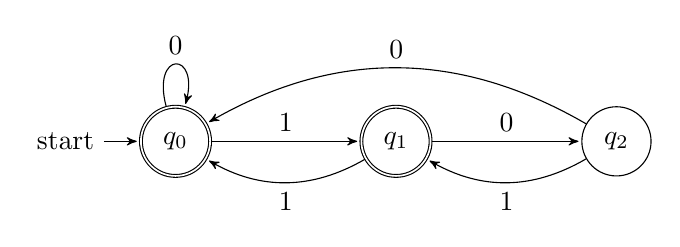
\begin{tikzpicture}[>=stealth',shorten >=1pt,auto,node distance=2.8cm]
 \node[initial,state,accepting] (q0) {$q_0$};
 \node[state,accepting] (q1) [right of=q0] {$q_1$};
 \node[state] (q2) [right of=q1] {$q_2$};

 \path[->] (q0)
 edge [loop above] node {0} (q0)
 edge node {1} (q1)
 (q1)
 edge node [above] {0} (q2)
 edge [bend left] node {1} (q0)
 (q2)
 edge [bend right] node [above] {0} (q0)
 edge [bend left] node {1} (q1);
 \end{tikzpicture}
 \caption{第一题}
\end{figure}

\section{第二题}
L = $\{ w \in {\{0, 1\}}^* | $ w contains both 01 and 10 as substrings $ \}$.

\begin{figure}[htbp]
 \centering
 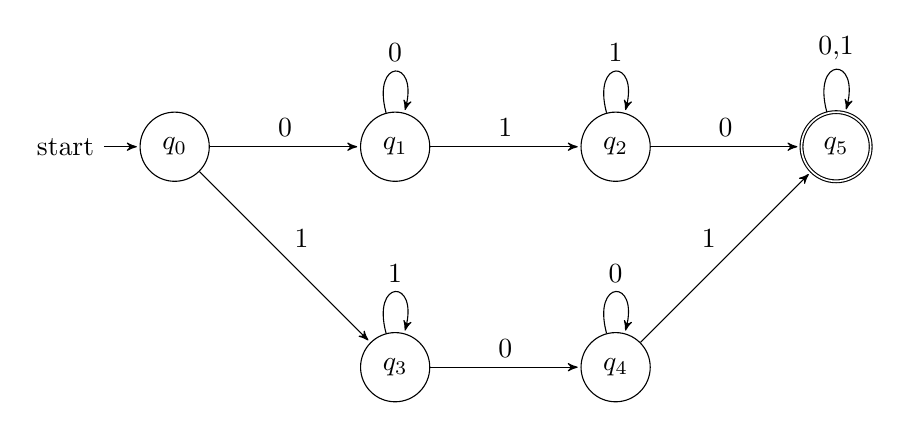
\begin{tikzpicture}[>=stealth',shorten >=1pt,auto,node distance=2.8cm]
 \node[initial,state] (q0) {$q_0$};
 \node[state] (q1) [right of=q0] {$q_1$};
 \node[state] (q2) [right of=q1] {$q_2$};
 \node[state,accepting] (q5) [right of=q2] {$q_5$};
 \node[state] (q3) [below of=q1] {$q_3$};
 \node[state] (q4) [below of=q2] {$q_4$};
 \path[->] (q0)
 edge node {0} (q1)
 edge node {1} (q3)
 (q1)
 edge [loop above] node {0} (q1)
 edge node {1} (q2)
 (q2)
 edge [loop above] node {1} (q2)
 edge node {0} (q5)
 (q3)
 edge [loop above] node {1} (q3)
 edge node {0} (q4)
 (q4)
 edge [loop above] node {0} (q4)
 edge node {1} (q5)
 (q5)
 edge [loop above] node {0,1} (q5);
 \end{tikzpicture}
 \caption{第二题}
\end{figure}

\section{第三题}
The set of all strings such that
each block of three consecutive symbols contains at least two 0’s.

\begin{figure}[htbp]
 \centering
 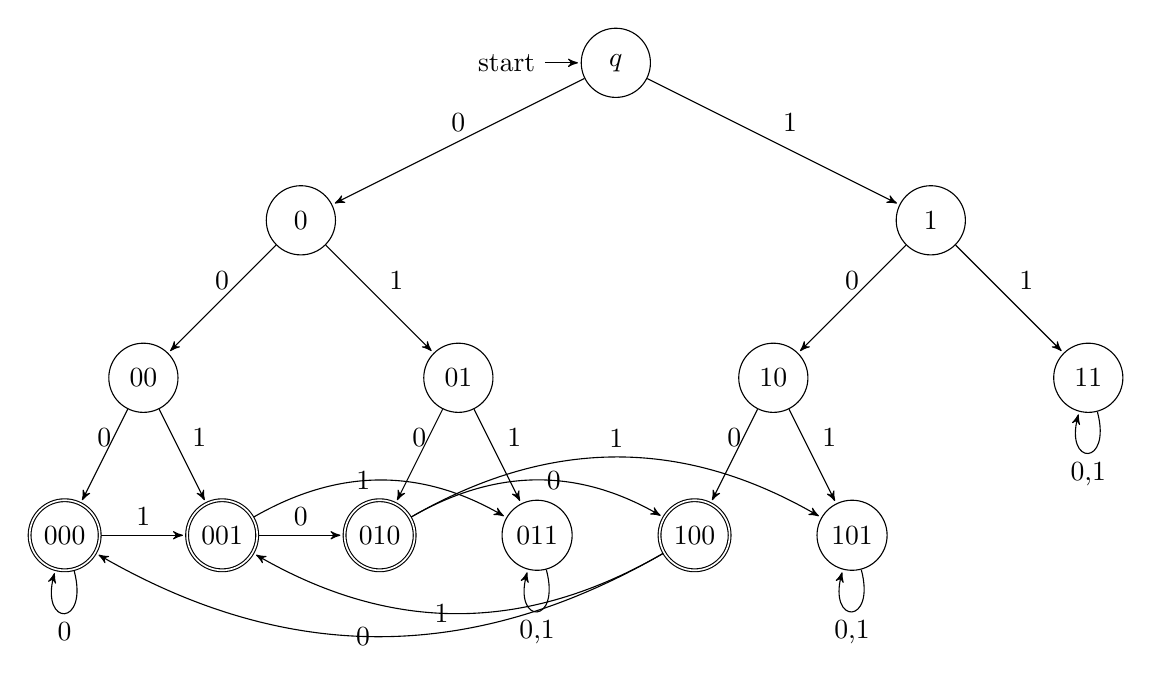
\begin{tikzpicture}[>=stealth',shorten >=1pt,auto]
 \node[initial,state] (q) at (7, 6){$q$};
 \node[state] (0) at (3, 4) {$0$};
 \node[state] (00) at (1, 2) {$00$};
 \node[state,accepting] (000) at (0, 0) {$000$};
 \node[state,accepting] (001) at (2, 0) {$001$};
 \node[state] (01) at (5, 2) {$01$};
 \node[state,accepting] (010) at (4, 0) {$010$};
 \node[state] (011) at (6, 0) {$011$};
 \node[state] (1) at (11, 4) {$1$};
 \node[state] (10) at (9, 2) {$10$};
 \node[state,accepting] (100) at (8, 0) {$100$};
 \node[state] (101) at (10, 0) {$101$};
 \node[state] (11) at (13, 2) {$11$};

 \path[->] (q)
 edge node [above] {0} (0)
 edge node {1} (1)
 (0)
 edge node [above] {0} (00)
 edge node {1} (01)
 (00)
 edge node [above] {0} (000)
 edge node {1} (001)
 (000)
 edge [loop below] node {0} (000)
 edge node {1} (001)
 (001)
 edge node {0} (010)
 edge [bend left] node [left] {1} (011)
 (01)
 edge node [above] {0} (010)
 edge node {1} (011)
 (010)
 edge [bend left] node [right] {0} (100)
 edge [bend left] node {1} (101)
 (011) edge [loop below] node {0,1} (011)
 (1)
 edge node [above] {0} (10)
 edge node {1} (11)
 (10)
 edge node [above] {0} (100)
 edge node {1} (101)
 (100)
 edge [bend left] node [left] {0} (000)
 edge [bend left] node [left] {1} (001)
 (101) edge [loop below] node {0,1} (101)
 (11) edge [loop below] node {0,1} (11);
 \end{tikzpicture}
 \caption{第三题}
\end{figure}

\section{第四题}
The set of strings such that
the number of 0's is divisible by 3, and the number of 1's is divisible by 2.

\begin{figure}[htbp]
 \centering
 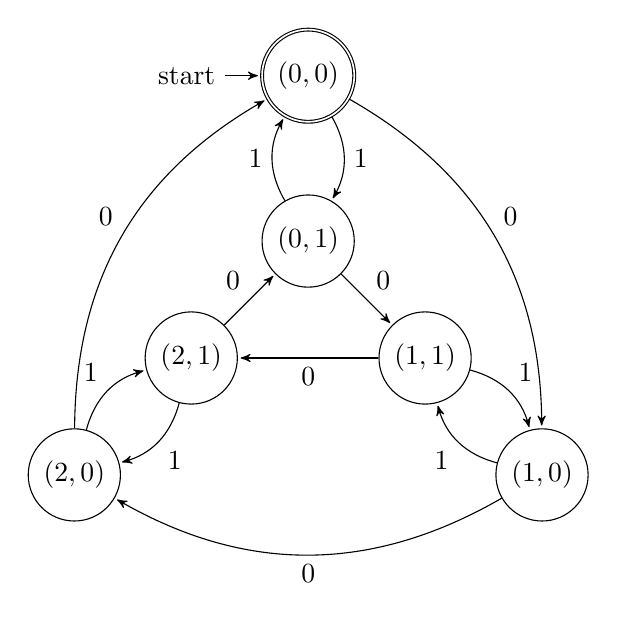
\begin{tikzpicture}[>=stealth',shorten >=1pt,auto,node distance=2.1cm]
 \node[initial,state,accepting] (00) {$(0, 0)$};
 \node[state,below of=00] (01) {$(0, 1)$};
 \node[state,below left of=01] (21) {$(2, 1)$};
 \node[state,below right of=01] (11) {$(1, 1)$};
 \node[state,below left of=21] (20) {$(2, 0)$};
 \node[state,below right of=11] (10) {$(1, 0)$};

 \path[->] (00)
 edge [bend left] node {0} (10)
 edge [bend left] node {1} (01)
 (10)
 edge [bend left] node {0} (20)
 edge [bend left] node {1} (11)
 (20)
 edge [bend left] node {0} (00)
 edge [bend left] node {1} (21)
 (01)
 edge node {0} (11)
 edge [bend left] node {1} (00)
 (11)
 edge node {0} (21)
 edge [bend left] node {1} (10)
 (21)
 edge node {0} (01)
 edge [bend left] node {1} (20);
 \end{tikzpicture}
 \caption{第四题}
\end{figure}

\section{第五题}
Design an NFA within four states for the language ${\{0\}}^* \cup {\{01\}}^*$.
\begin{figure}[htbp]
 \centering
 \begin{tikzpicture}[>=stealth',shorten >=1pt,auto,node distance=3cm]
 \node[initial,state,accepting] (S0) {$S_0$};
 \node[state,accepting,above right of=S0] (S1) {$S_1$};
 \node[state,below right of=S0] (S2) {$S_2$};
 \node[state,accepting,right of=S2] (S3) {$S_3$};

 \path[->] (S0)
 edge node {$\varepsilon$} (S1)
 edge node [below] {0} (S2)
 (S1) [loop above] edge node {0} (S1)
 (S2) [bend left] edge node {1} (S3)
 (S3) [bend left] edge node {0} (S2);
 \end{tikzpicture}
 \caption{第五题}
\end{figure}

\section{第六题}
Design an NFA for the following language over
$ \Sigma = \{0, 1\}, L = \{w | w$ contains at least two 0's or exactly two 1's $\}$.
\begin{figure}[htbp]
 \centering
 \begin{tikzpicture}[>=stealth',shorten >=1pt,auto,node distance=3cm]
 \node[initial,state] (S0) {$S_0$};
 \node[state,above right of=S0] (S1) {$S_1$};
 \node[state,right of=S1] (S2) {$S_2$};
 \node[state,accepting,right of=S2] (S3) {$S_3$};
 \node[state,below right of=S0] (S4) {$S_4$};
 \node[state,right of=S4] (S5) {$S_5$};
 \node[state,accepting,right of=S5] (S6) {$S_6$};

 \path[->] (S0)
 edge node {$\varepsilon$} (S1)
 edge node [below] {$\varepsilon$} (S4)
 (S1) edge node {0} (S2)
 (S2) edge node {0} (S3)
 (S4) edge node {1} (S5)
 (S5) edge node {1} (S6)
 (S1) [loop above] edge node {1} (S1)
 (S2) [loop above] edge node {1} (S2)
 (S3) [loop above] edge node {0,1} (S3)
 (S4) [loop below] edge node {0} (S4)
 (S5) [loop below] edge node {0} (S5)
 (S6) [loop below] edge node {0} (S6);
 \end{tikzpicture}
 \caption{第六题}
\end{figure}

\end{document}
